\documentclass[journal, a4paper]{IEEEtran}


\usepackage{graphicx}   
\usepackage{url}     
\usepackage{multicol}
\usepackage{amsmath}  
\usepackage{graphicx}
\usepackage{xcolor}
\usepackage[export]{adjustbox}
\usepackage{verbatim}


\begin{document}
    \twocolumn[
    \begin{@twocolumnfalse}
	\title{Multiplexed Spectral Imaging with a High-Flux 330-$\mu$m Pitch Cadmium Zinc Telluride (CZT) Detector}
	\author{Chelsea A. S. Dunning, Spencer M. Robinson, Jericho O'Connell, Kevin J. Murphy, Kris Iniewski, and Magdalena Bazalova-Carter }
	\maketitle

\section{Abstract}
Spectral computed tomography (sCT) imaging with a high-flux cadmium zinc telluride (CZT) detector of a phantom with three contrast materials is presented. The table-top sCT imaging system consisted of a diagnostic x-ray tube, rotation stage for phantom placement, a translation stage to enable detector motion and a 330-$\mu$m pitch CZT detector of 8$\times$12 mm in size capable of using six energy bins. The 3D-printed 3-cm diameter phantom contained six 5-mm diameter vials with 1\% and 5\% solutions of iodine, gadolinium and gold. The phantom was imaged with 120$\,$kVp 1$\,$mA beam with a 1-mm aluminum filter using 180 rotation steps in 2$^\circ$ intervals. Each detector data acquisition took 1$\,$s and the entire spectral CT scan resulted in a mean imaging dose of 172 mGy. 

    \newline
    \end{@twocolumnfalse}]
\section{Introduction}
\PARstart{T}{he} use of energy-selective x-ray computed tomography (CT) for material analysis was proposed in the 1970s\cite{alvarez1976energy}. Energy-selective CT imaging has been recently applied in the form of dual-energy CT (DECT) imaging, in which the effective atomic number of each material can be reconstructed and used for a more accurate material analysis compared to conventional x-ray CT. Many studies have employed DECT for this purpose\cite{silva2011dualab,yu2012dual,johnson2007matdiffDECT}. DECT is performed by scanning with two different x-ray beam energies to create two separate images which are then subtracted to enhance the material of interest. This presents a number of challenges in terms of imaging time, subject motion, and imaging dose. In addition, DECT is often limited to distinguishing materials with very different attenuation curves, such as bone and soft-tissue\cite{fornaro2011review}. Thanks to the recent advancements in photon-counting detector development, multi-energy x-ray imaging, or spectral CT, has become possible using only one x-ray beam energy. Spectral CT imaging is capable of distinguishing multiple high-atomic number (\textit{Z}) materials by selecting appropriate energy bins above and below the K-edges of each material on a photon-counting detector capable of energy discrimination. In DECT imaging, a similar effect is achieved by selecting appropriate x-ray beam energies on either side of a K-edge for one material. It is anticipated that spectral CT will lead to important enhancements in contrast visualization, lower imaging dose, and reduced image artifacts. However, detector optimization as well as image reconstruction techniques cause spectral CT to lag behind conventional photon-integrating x-ray imaging. The purpose of this study was to start bridging that gap. 

In this study, the goal is to simultaneously image three clinically-relevant high-\textit{Z} contrast agents, namely iodine, gadolinium, and gold, using spectral CT. Iodine is a routinely-used contrast agent for many clinical CT scans. Gadolinium, while typically used as a contrast agent in magnetic resonance imaging (MRI) scans, also has been used in CT imaging \cite{taguchi2015imaging, bennett2014hybrid, si2018multicolour, feuerlein2008multienergy}. Finally, with the use of biocompatible gold nanoparticles for possible dose enhancement\cite{hainfeld} and drug delivery\cite{ghosh2008gold} in cancer treatment, gold is an attractive contrast agent for CT imaging. Spectral CT imaging has been used to simultaneously image both gadolinium and iodine contrast agents using a Medipix silicon spectral detector\cite{bennett2014hybrid} and a CdTe detector array\cite{schlomka2008experimental}. However, due to the absorption efficiency of silicon at higher x-ray energies compared to CZT, the Medipix detector may struggle to image higher-\textit{Z} materials such as gold. In addition, CdTe detectors suffer from low count rates compared to CZT detectors, which is not ideal for medical CT scans. Recently iodine, gadolinium, and gold have been imaged before in a single multi-energy spectral CT study using six energy bins on a semi-conducting detector, although at most only two contrast agents were imaged simultaneously with a pencil beam geometry\cite{si2018multicolour}. This study demonstrates faster simultaneous spectral CT and conventional cone beam CT of iodine, gadolinium, and gold inside a small animal phantom using a high-flux, photon-counting CZT detector for the first time.

****ROUGH NOTES****
- find iodine image without gold -> when I showed the image that didn't have gold, in the "raw" units it was a dark "hole" rather than bright. Upon normalizing to HU post-subtraction I get a similar image as Jericho. Gold has an extremely high density, nearly quadruple that of iodine. I wonder if that effect is showing up in the HU normalized image?
- I think the introduction first draft is finished. What does everyone think? Should I add more information about how CZT photon-counting detectors work? -Chelsea


\section{Materials and Methods}

\subsection{Imaging setup}
\begin{center}
\begin{figure}[htbp]
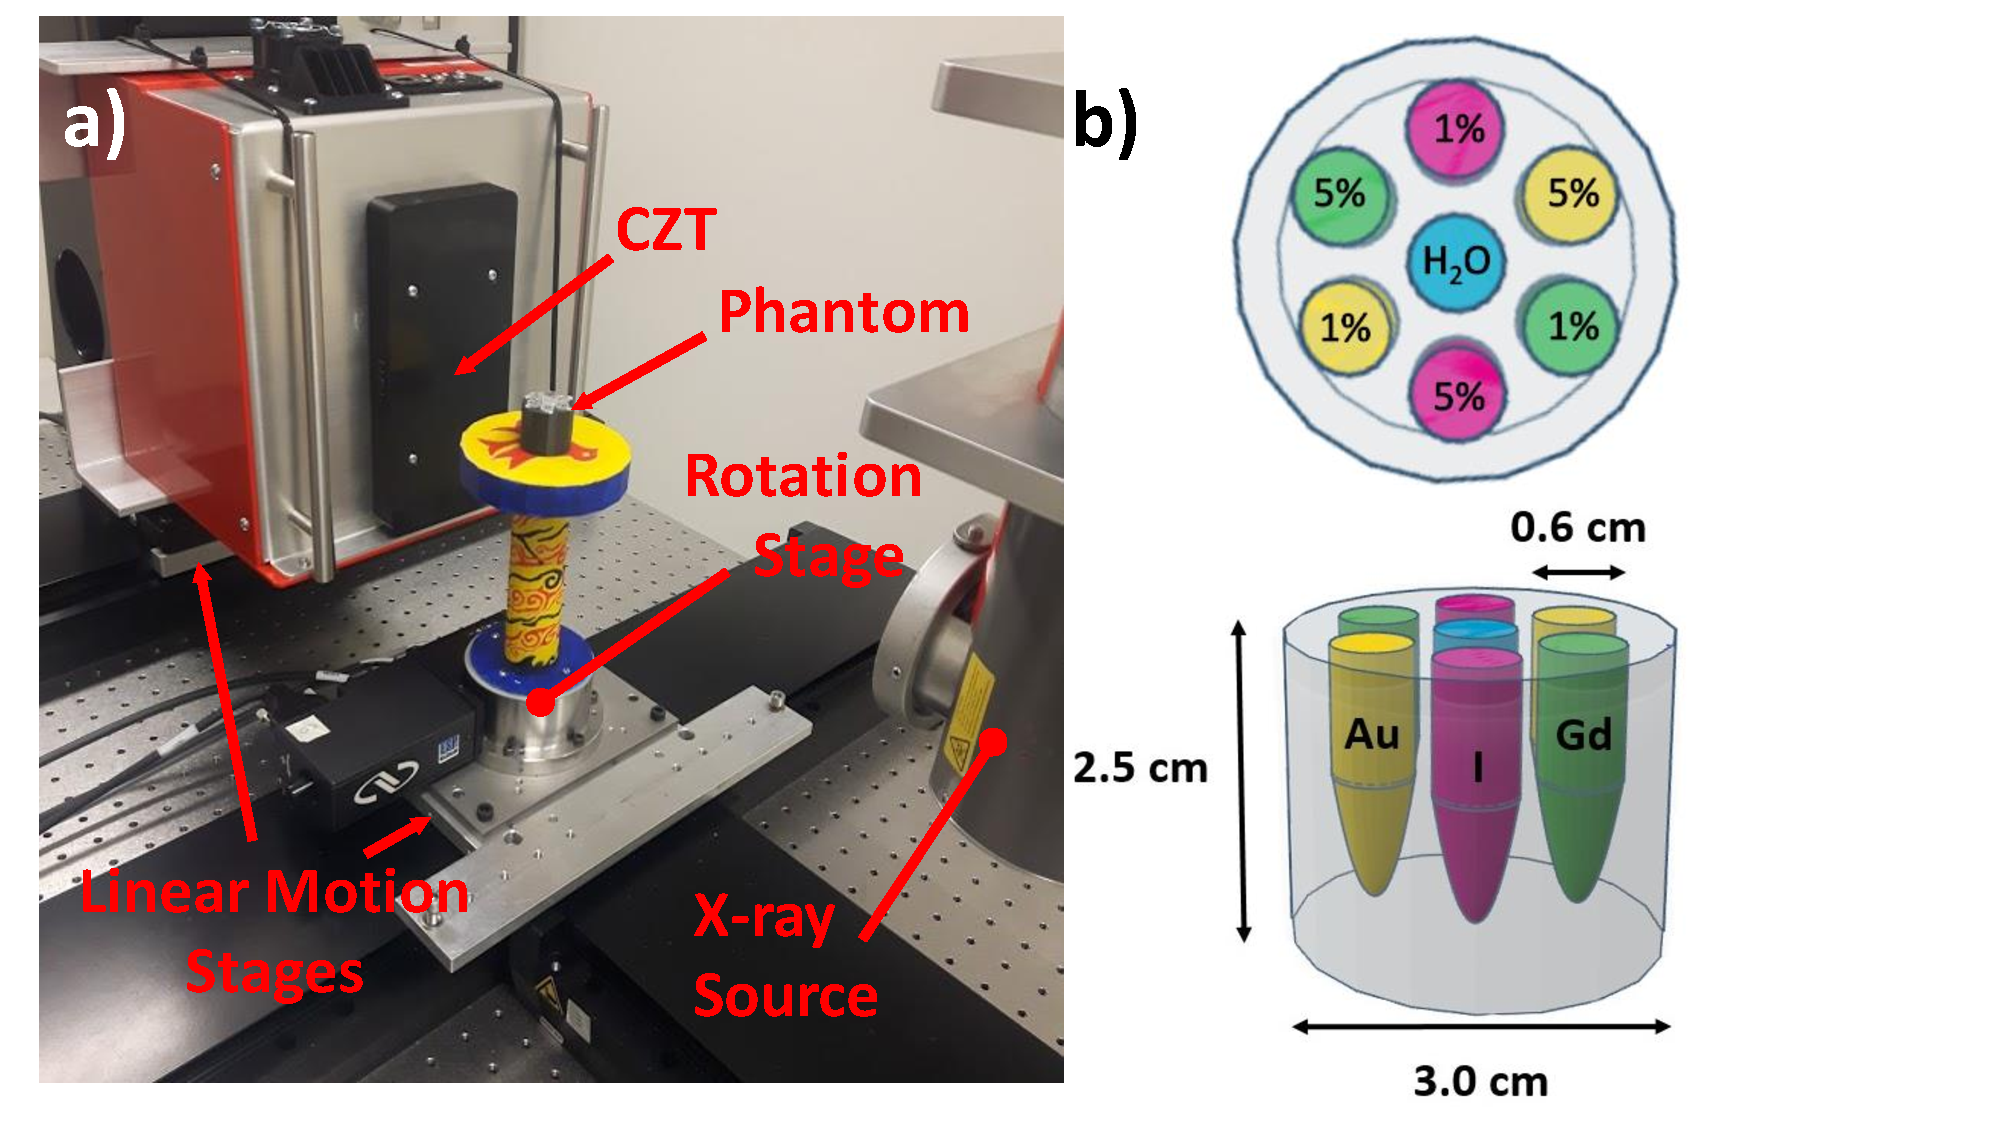
\includegraphics[width=\linewidth]{PhantomOrientation.pdf}
\caption{a) Lab set up for Spectral CT data acquisitions, with components labeled.  b) Contrast phantom holder with layout of concentrations for each contrast agent. }

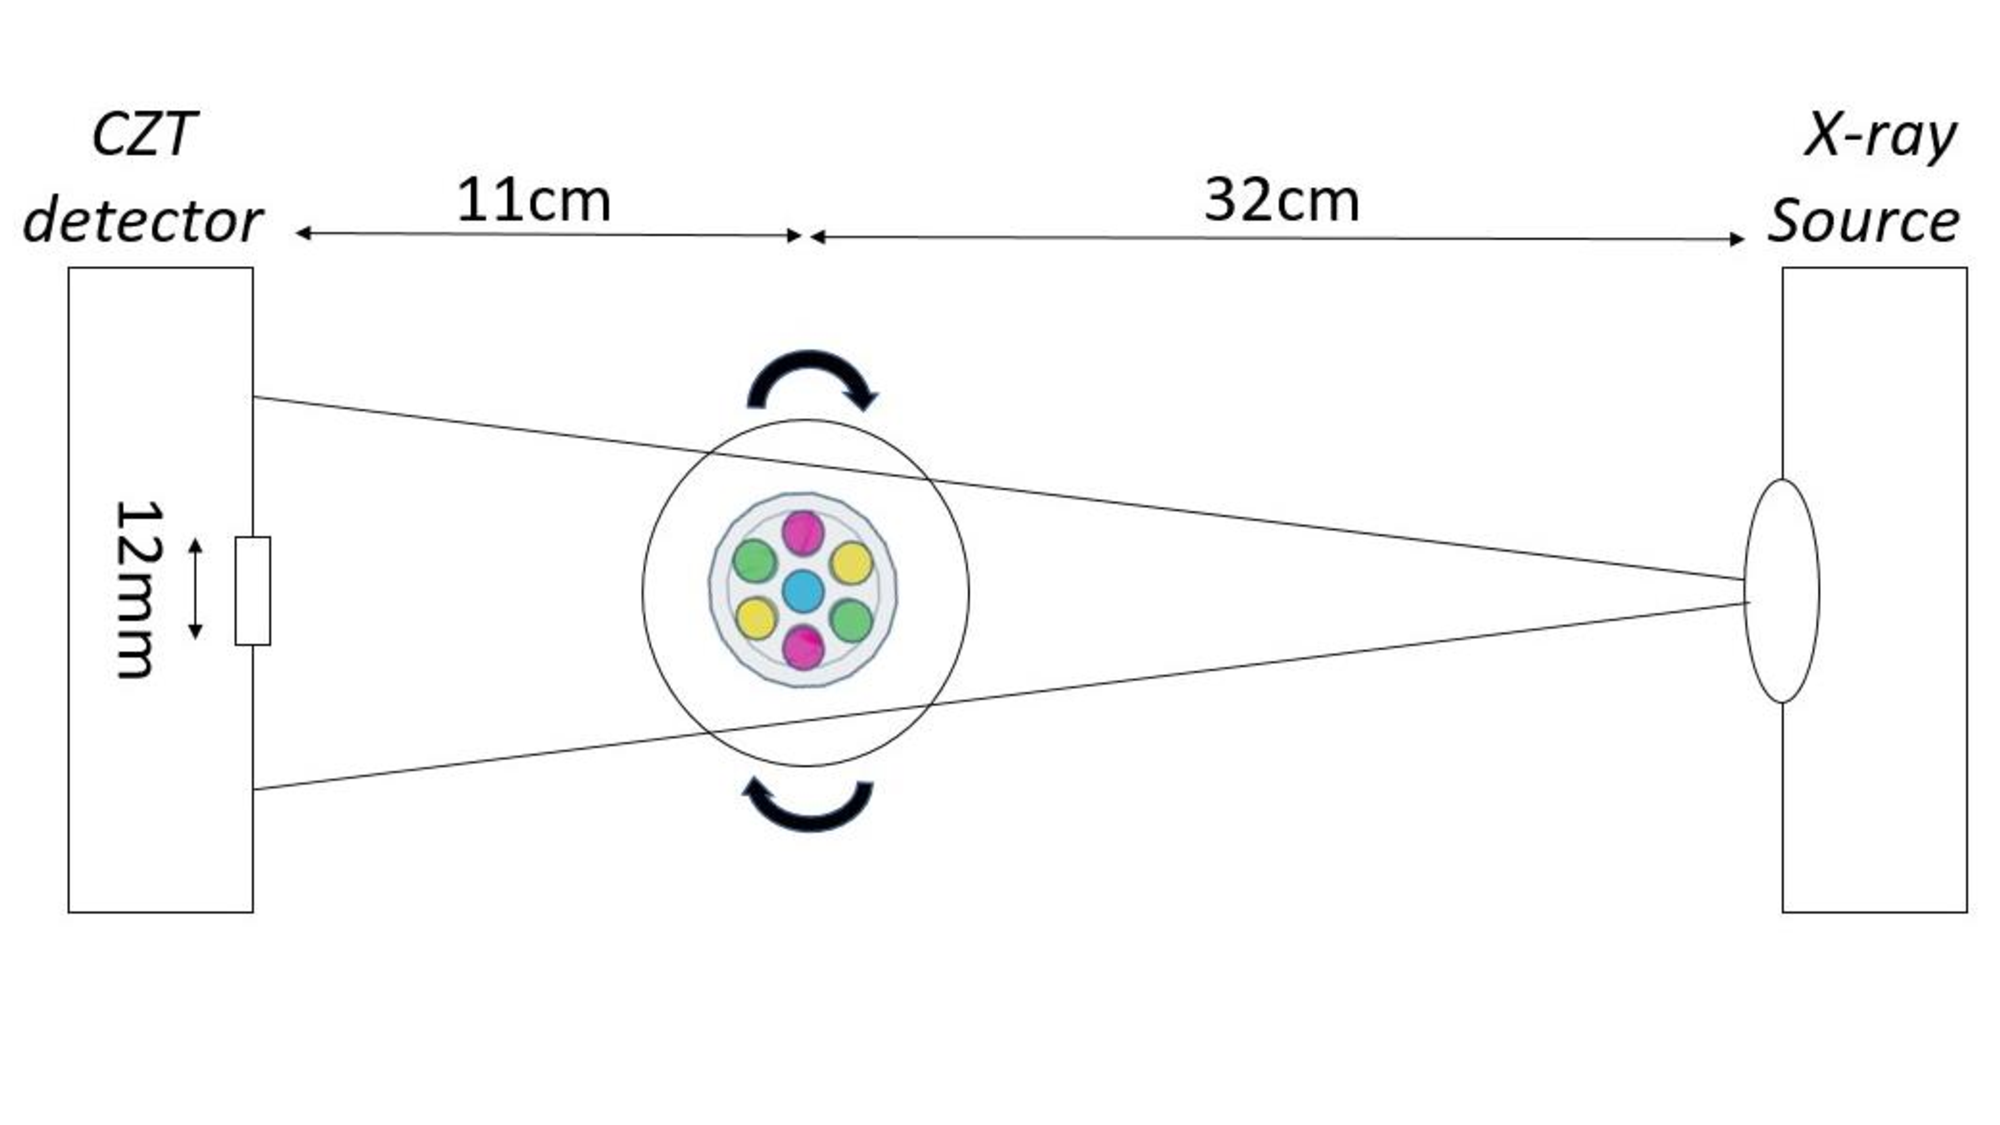
\includegraphics[width=\linewidth]{LabSchematic.pdf}
\caption{CZT spectral CT design schematic}
\label{imagingsetup}
\end{figure}
\end{center}


\subsection{Data acquisition}
Data acquisition was completed using a CZT detector of 8$\times$12 mm in size from Redlen Technologies. The CZT detector module uses 2 mm thick, 330$\mu$m pitch high-flux CZT sensor capable of operating at 250 Mcps/mm$^2$ rates without any signs of polarization. The CZT crystal is grown using the Traveler Heat Method (THM) by Redlen Technologies. The sensor is connected to the high-speed photon counting ASIC that operates at rates up to 62.5 Mcps per channel. The ASIC communicates through high-speed LVDS I/Os to the external PC via programmable FPGA. The energy of photons incident onto the detector are sorted into six energy bins by the ASIC. In the case of this experiment the energy bins were set to 16-33 keV, 33-41 keV, 41-50 keV, 50-64 keV, 64-81 keV, \& 81-120 keV. These values were used to accommodate for the K-edge values of the three contrast agents used, which are shown in Figure \ref{attencoeffs}.
\newline
\indent The CZT detector was mounted on a horizontal and a vertical linear motion stage from Newport Corporation. The X-ray source was a module XRS-160 from Comet Technologies. This X-ray source was mounted on two linear motion stages as well, one horizontal and perpendicular to the detectors motion stage and a vertical motion stage. Between the CZT detector and X-ray source was a rotation stage mounted on a horizontal motion stage parallel to the CZT detector. The phantom containing 1\% and 5 \% solutions of I, Gd, and Au as contrast agents was placed on this rotation stage and scanned 180 times over a 360$^\circ$ rotation to create a sinogram, 5 rotations were performed in order to image the entire phantom body. The I solution used was iodine-based Omnipaque 300 (iohexol, GE Health- care, Princeton, NJ), the Au solution used was Gold (III) Chloride solution from Nanopartz Inc (GG3CS-25.4-100 Lot AUY03-7077), and the Gd used was synthesized in the form of nanoparticles dispersed in hexanes\cite{gadolNPs}. All of these solutions were contained in 0.2 ml Fisherbrand Flat Cap PCR tubes, and diluted in 0.6 ml Axygen Microtubes.

\begin{figure}[htbp]
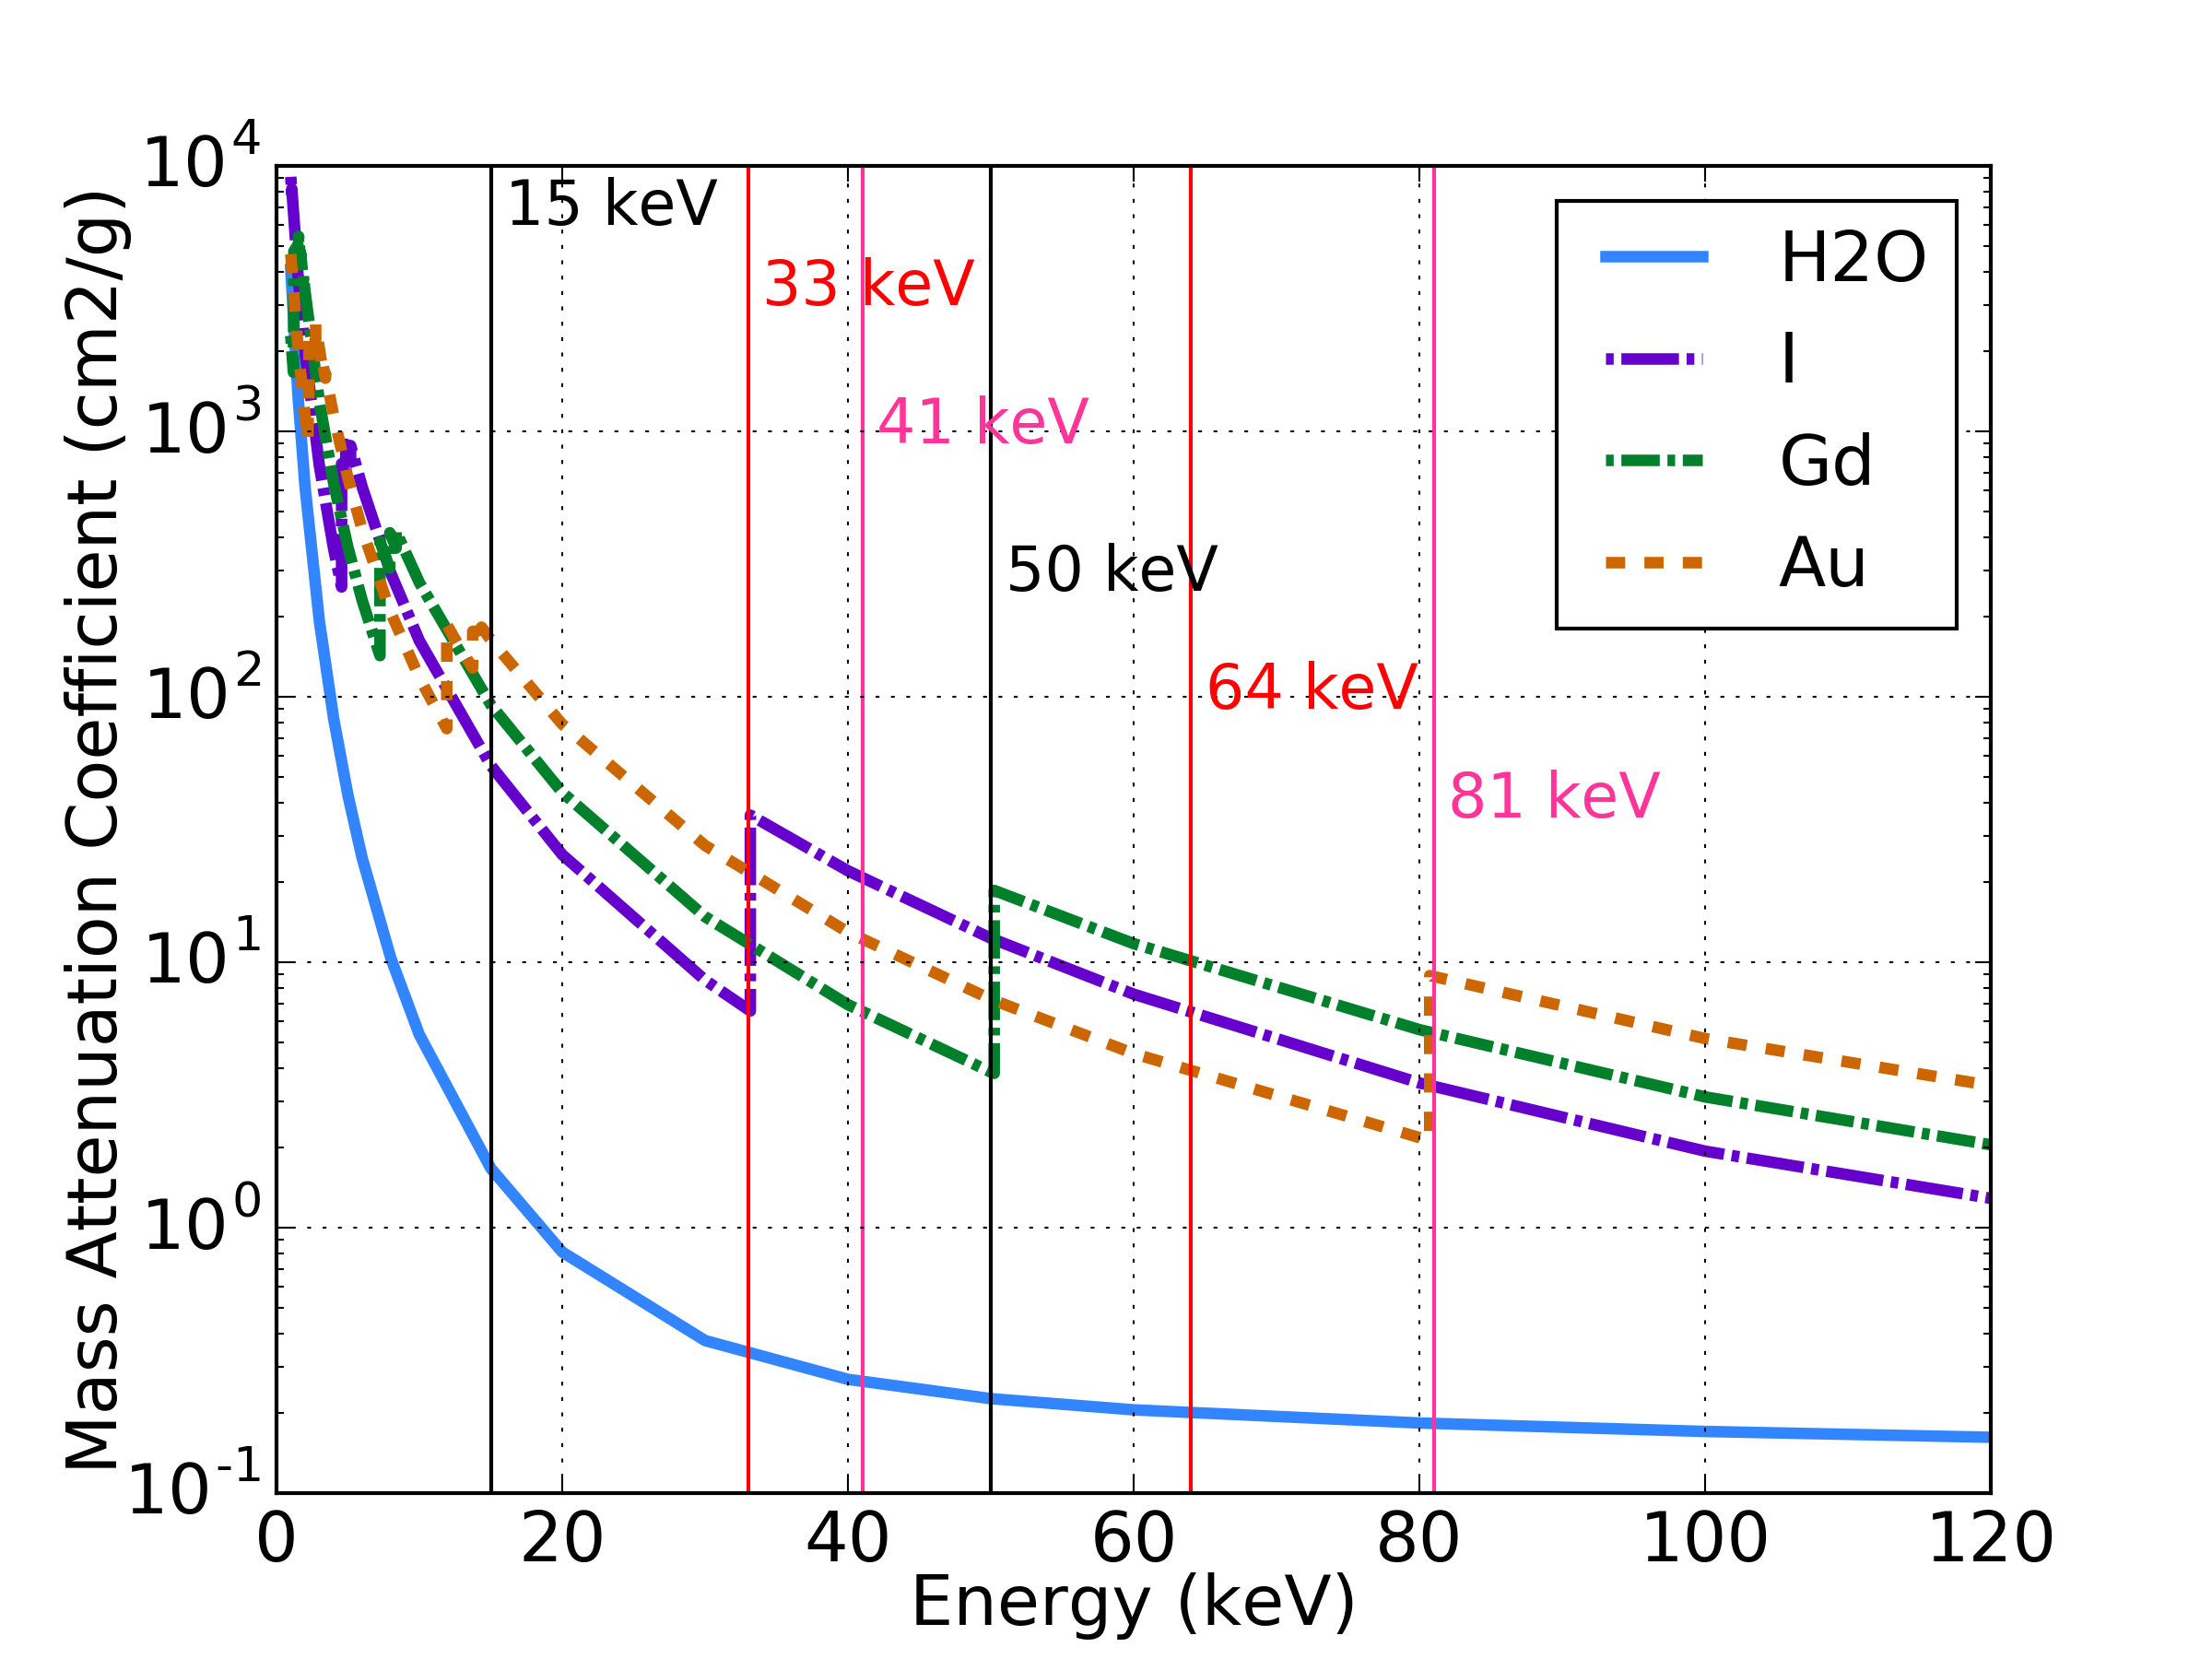
\includegraphics[width=\linewidth]{Figures/sCT_attencoeffs.png}
\caption{Mass attenuation coefficients of water, iodine, gadolinium, and gold shown with the thresholds of the energy bins on the CZT detector.}
\label{attencoeffs}
\end{figure}

The 0.2 ml PCR tubes were inserted into a 3D printed phantom made of solid polylactic acid (PLA) of density ???, the contrast agents were alternating as imaged in figure 1.b). The phantom was printed to reduce the air gap with the PCR tubes when inserted. The use of the Newport linear motion stages allowed for sub-micron accuracy in motion of the detector and X-ray source. This allowed for precise stitching of sinograms produced from the 5 360$^\circ$ rotations. For all scans of the phantom the X-ray source was running at 120 kVp, and 1 mA with a 1.0mm focal spot, and 1mm of Al filtration, while the detector was acquiring 1-s images with 4 equivalently spaced frames. Acquisition time for one full rotation of the phantom took 32 minutes, 5 rotations were done to image to whole phantom. 

\subsection{Dose Estimation}
To estimate the dose of the scan, the x-ray tube and a cylindrical phantom was simulated in TOPAS\cite{topas}, a GEANT-4 based Monte Carlo software package, in the same setup as shown in Figure \ref{imagingsetup}. The relevant physics modules were included, such as "g4em-standard\_opt4", "g4decay", "g4ion-binarycascade", "g4stopping", and "g4em-extra". In addition, the simulation of fluorescence, Auger electrons, and particle-induced x-ray emission were included. For simplicity, the phantom was assumed to be pure PLA and was only simulated for one rotation. The resulting dose per primary electron in the phantom volume from the simulation was $3.05 \times 10^{-19}$ Gy/primary. After multiplying by 180 rotation steps, the imaging time of 1 second per rotation, and the beam current of 5 mA, then dividing by the electric charge of an electron, the mean estimated dose to the phantom was calculated to be 172 mGy.

\subsection{Image Reconstruction}

\subsubsection{Spectral Image Reconstruction}

Due to the limited size of the detector, image acquisition included multiple $360^o$ rotations of the phantom with the detector translated to capture the whole phantom. The detector was moved five times with positioned defined relative to the X-Ray tube of -30, -21, -12, -3 and 6 mm respectively. Thus, to generate one reconstruction there were five sets of 180 projections that were combined as sinograms to make a single reconstruction.
MATLAB (The Mathworks, Natick, MA) was used for data processing and image reconstruction, while Python was used for data analysis. For each offset relative to the X-Ray tube an air-image was taken, the counts were converted into projections as $p = -ln(I/I_0)$ where $I$ is the number of counts and $I_0$ is the number of counts in the air-image. The five different sets of sinograms were cropped and stitched together to cover the whole phantom. 
Images underwent ring-artifact corrections using the wavelet method\cite{munch2009stripe}. This method was used to remove both vertical and horizontal stripes from the image to account for the non-uniformity of the pixel response. CT images were then reconstructed using filtered back-projection with a Hamming filter. 

\subsubsection{K-Edge Images}

The K-edge imaging was performed by subtracting the energy bin directly above the k-edge from the bin directly below the K-edge in one axial CT slice of the phantom. The subtraction of the two energy bins was done after the reconstruction process. This method produced three K-edge images, one for each of Iodine, Gadolinium, and Gold. The K-edge energies for these three elements were considered to be 33.2 keV, 50.2 keV, and 80.7 keV  respectively. Contrast to noise ratio (CNR) was evaluated for a region of interest (ROI) by calculating the ratio of contrast (the difference between mean values of the ROI and the phantom body) and the standard deviation of the signal in the phantom body which can be seen in Fig. \ref{colour_plots}. To better visualize the K-edge images, all pixels were scaled by the mean value of the ROI for the 5\% concentration to make intensity proportional concentration of contrast agent.


\begin{figure}[htbp]

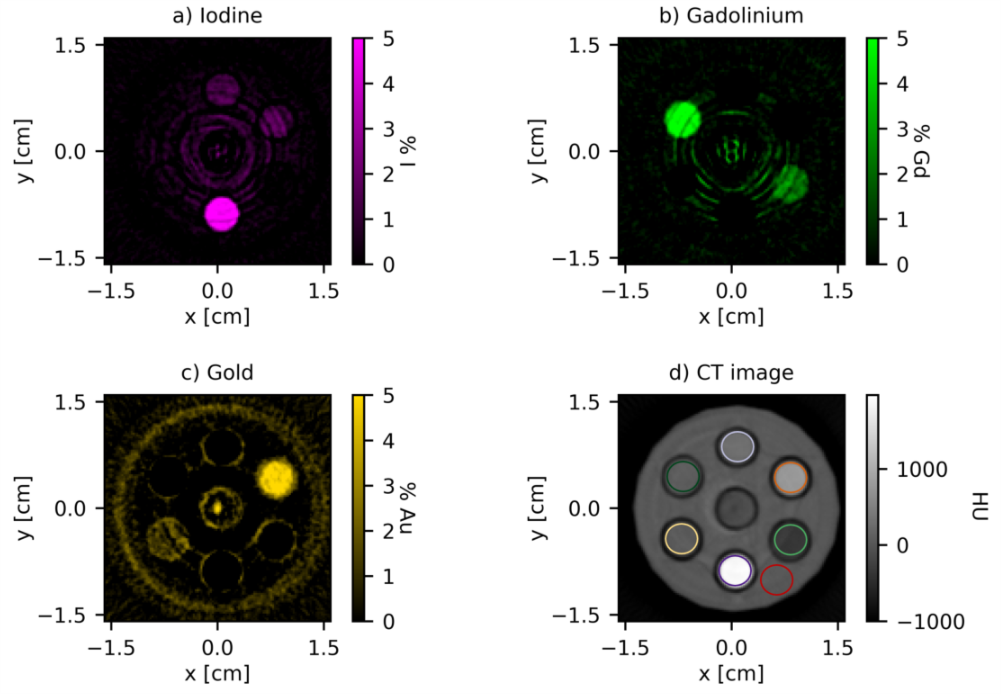
\includegraphics[width=\linewidth]{Figures/individual_kedge.png}

\caption{Each image is one axial slice of the CT reconstruction: a) The first K-edge image isolating iodine, b) the second K-edge image isolating Gadolinium and finally c) the third K-edge image isolating Gold. Subplot d) is the summed reconstruction over all of the energy bins, the circles in the image represent the ROIs taken from the image to generate the CNR, the red circle is the ROI used to define the contrast to noise ratio.}
\label{colour_plots}

\end{figure}


\section{Results}

\subsection{CT Images}

Fig. \ref{colour_plots} shows the results of the K-edge subtraction technique. The top image is the reconstruction of all energy bins as reference for the image quality that can be expected from the detector. The 5\% Iodine has very high contrast in this image as well as the 5\% gold which easily stands out from the body of the phantom. However the other inserts are hard to differentiate from the phantom body. 

Throughout the image reconstruction process ring artifacts were seen in the K-edge images as can be seen in the middle two K-edge reconstructions of Iodine and Gadolinium.

The Iodine K-edge image created by subtracting the 33-41 keV from the 16-33 keV energy bin is seen in the second image, assigned a purple colormap in Fig. \ref{colour_plots}. The 5\% iodine insert stands out clearly from the rest of the image, however the 1\% iodine is not clearly differentiated from the PLA background nor from the Gold insert. The Gadolinium K-edge reconstruction in Fig. \ref{colour_plots} is assigned a green colormap. In this case both the 5\% and the 1\% Gadolinium inserts had good contrast relative to the phantom body. This is similar to the Gold K-edge reconstruction where the two gold inserts stand out relative to the phantom body. However, the CNR results show that the contrast of the 1\% inserts are not all above the Rose criterion \cite{rose}.

\begin{figure}[h!]
\centering
\adjincludegraphics[width=\linewidth,trim={1cm 3cm 1cm 3cm},clip]{Figures/Composite_Image.pdf}

\caption{a) Shows the CT image for reference. b) Shows reconstructed RGB using the reconstruction of all of the energy bins with an RGB created by assigning an gold colormap to Gold, green to Gadolinium and purple to Iodine. All of the K-edge images are scaled between 0 and 5\% concentration of contrast agents. c) is the composite of the two images.}
\label{rgb_image}

\end{figure}

An optimal way of visualizing the results of multiplex imaging is to assign the different K-edge images to the three channels of an RGB image. In Figure \ref{rgb_image} this method can be seen overlayed on the summed energy bins to display all the contrast agents in one image. A confounding factor is the background noise in the phantom body which is seen to be prevalent in the overlayed image (right).

\subsection{Contrast-to-Noise Ratio}

CNR of K-edge images and individual energy bins are presented in Fig. \ref{contrast_all} (second and third columns). As expected, CT reconstructions of the inserts with high attenuation resulted in high CNR. The Iodine insert having the highest CNR as is evident in Fig. \ref{rgb_image}.

In general, CNR in the K-edge images (first column) was higher than the Rose criterion (red line), 11.5, 14.5, and 6.9 respectively for the Gold, Gadolinium and Iodine respectively. However for the 1\% cases CNR were 2.0, 11.3 and 3.0 respectively for the Gold, Gadolinium and Iodine. The Gadolinium, with a CNR above 4 is thus the only detectable contrast agent at 1\%.

\begin{figure}[!h]

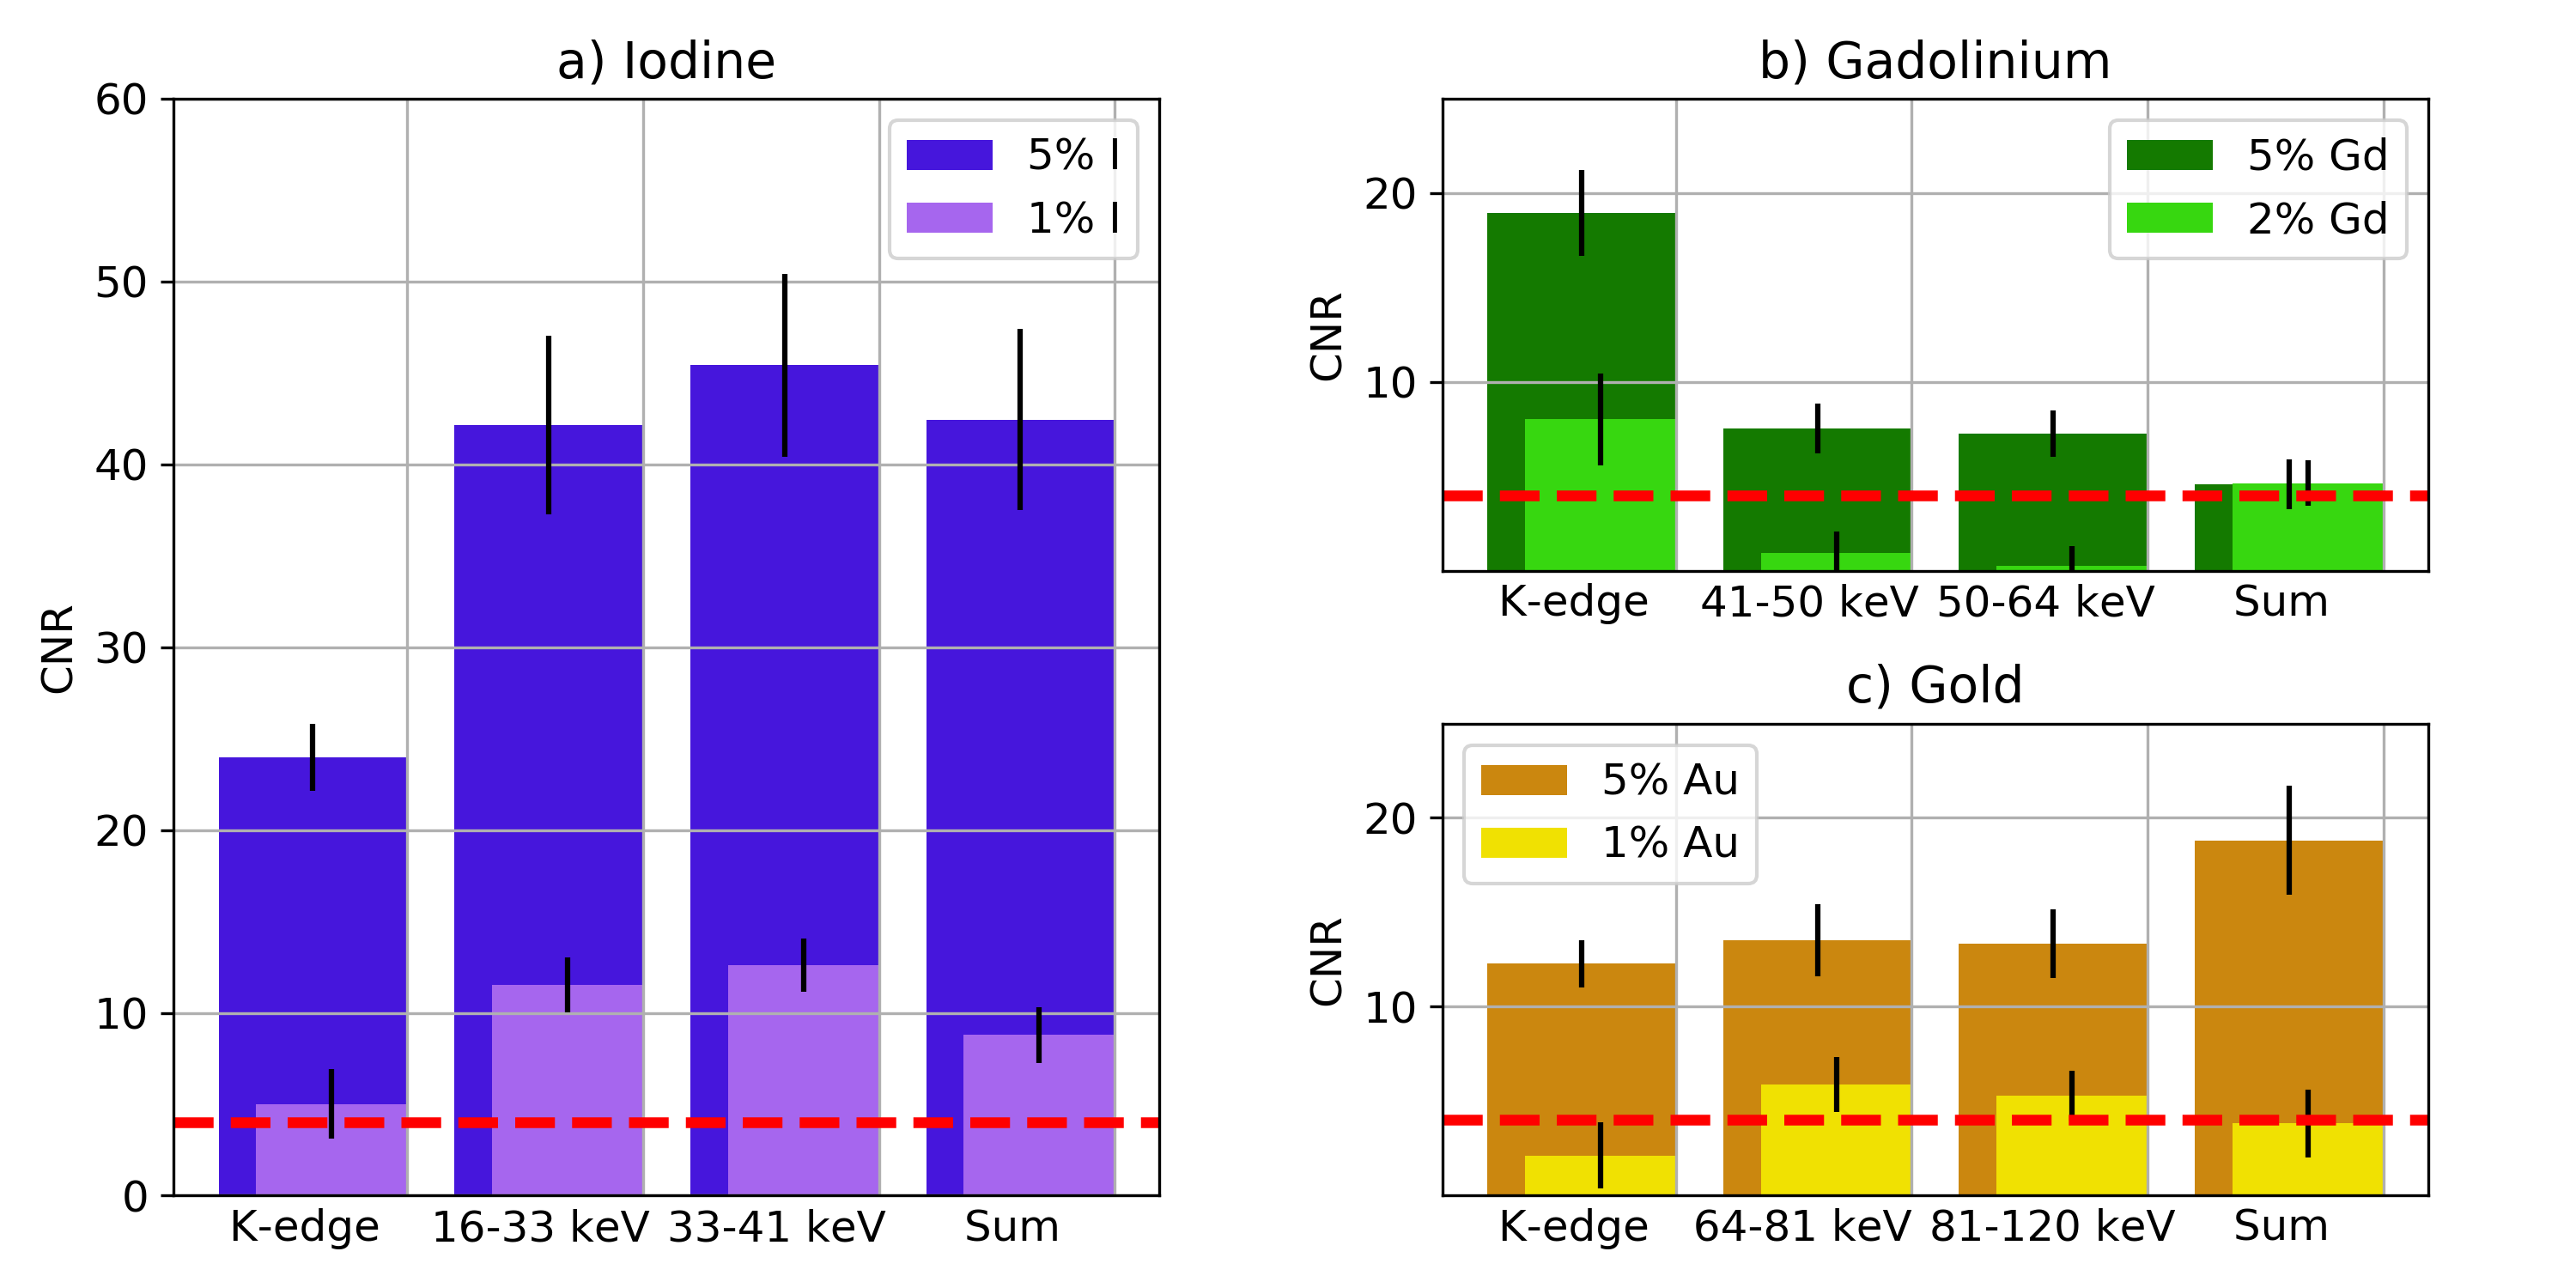
\includegraphics[width=\linewidth]{Figures/contrast_all.png}

\caption{The CNR results for the K-edge images as well as the bins used to construct the images for comparison. The red line denotes the limit of human vision at a CNR value of 4.}
\label{contrast_all}

\end{figure}

The scaling relation between the concentrations of contrast agents in the phantom was largely consistent with the signal intensities in the ROIs as seen in Fig. \ref{concentrations}. For Iodine, a) in Fig. \ref{concentrations}, the average concentration over all slices in the 1\% and 0\% ROIs showed slightly higher signals than expected at 1.15\% and 0.09\% respectively. The Gadolinium ROIs were both within one standard deviation of the theoretical values at 2.06\% and 0.02\% respectively for the 2\% and 0\% ROI. The 2\% Gadolinium ROI had a larger standard deviation than all other ROIs and its concentration showed dependence on phantom depth, with lower values at the bottom of the phantom, as can be seen in Fig \ref{concentrations} b). The 1\% Gold ROI in Fig. \ref{concentrations} c), was within one standard deviation with a value of 1.01\%, however the 0\% region was not with a value of -0.13\%.

\begin{figure}[!h]

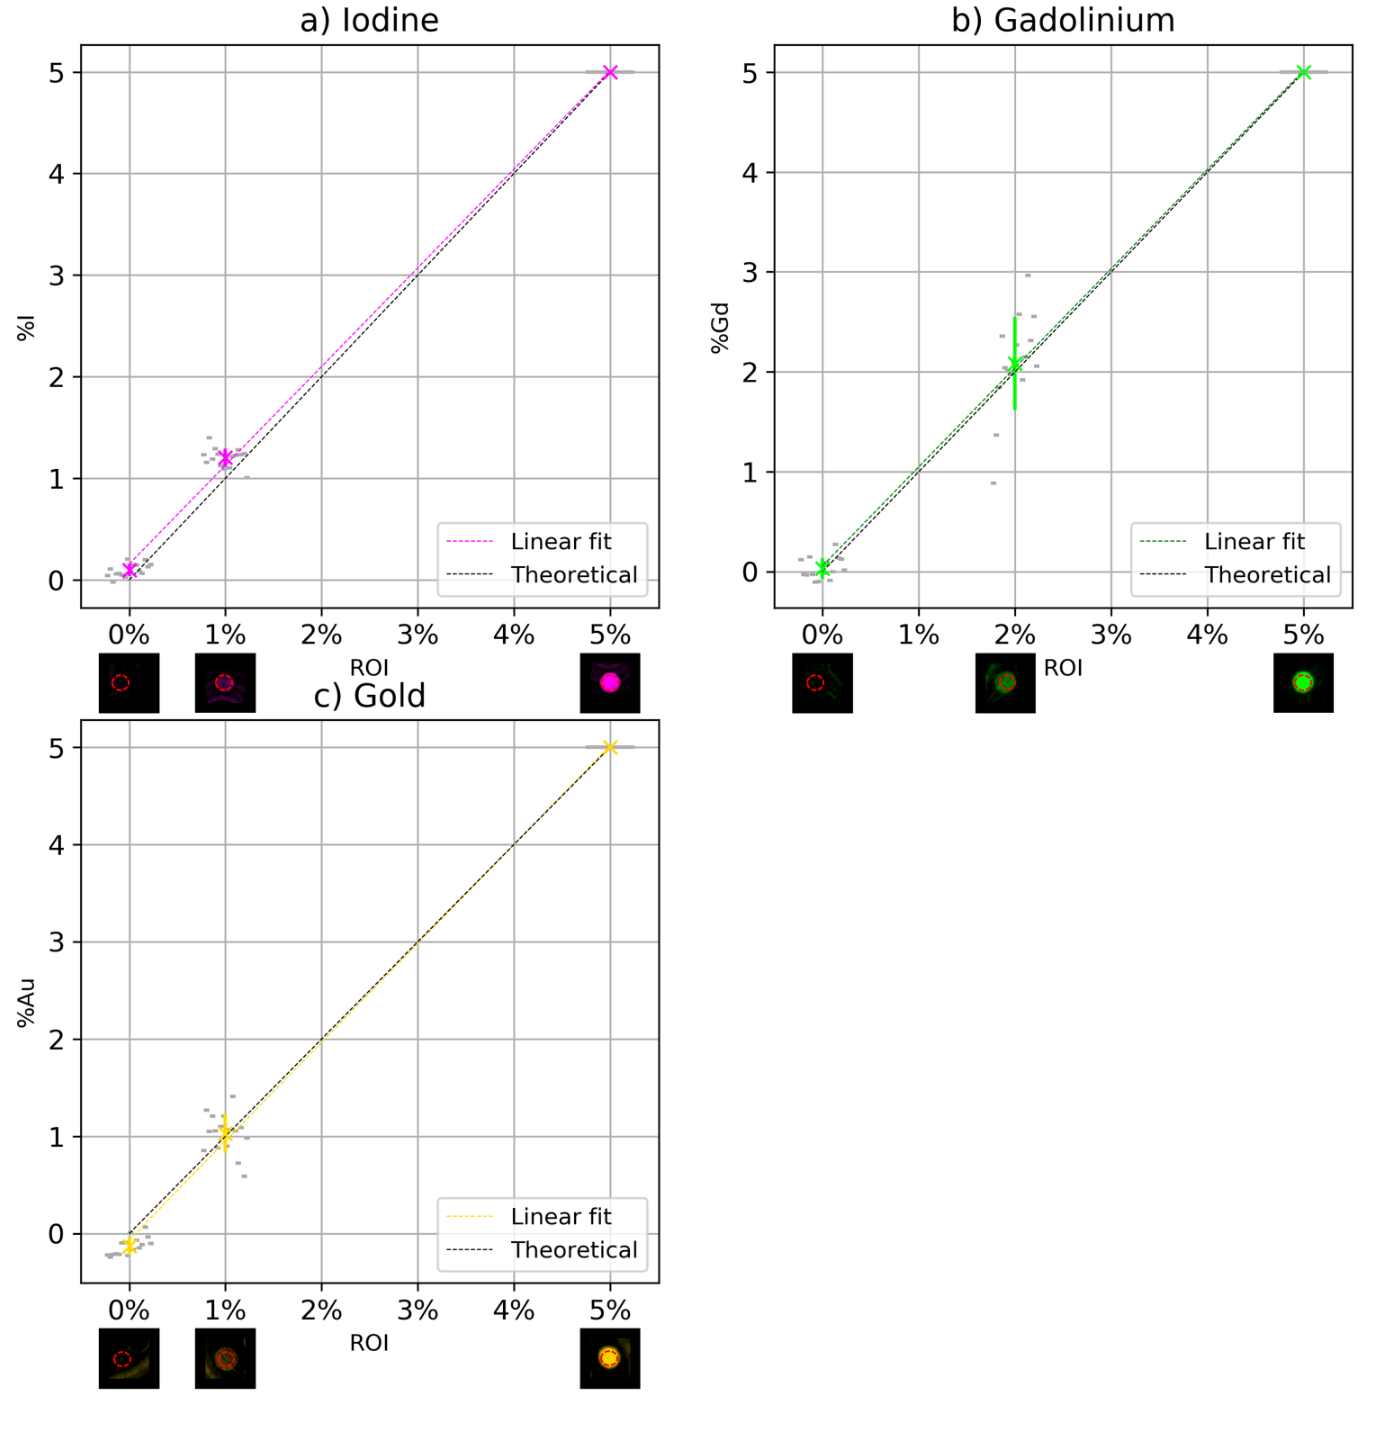
\includegraphics[width=\linewidth]{Figures/concentrations.png}

\caption{The contrast agent concentrations over all slices are shown. The average concentration of the ROIs is plotted as a coloured x with error-bars representing one standard deviation, the grey lines around the x denoting the individual slices. Each grey line is assigned a horizontal offset according to its location in the phantom; the farther left the line the lower the slice is in the phantom. Thumbnails show a sample ROI in red. Finally, a colored line of best fit is plotted as well as the theoretical line of best fit shown in black.  }
\label{concentrations}

\end{figure}

\section{Discussion}
We have showcased conventional and K-edge CT imaging of three high-\textit{Z} contrast agents simultaneously in a 3D-printed small animal phantom using a CZT photon-counting detector. However, there were a few factors that affected the results. 

The energy bin thresholds on the CZT detector were chosen to ensure roughly the same relative number of incident x-rays from the 120 kVp source were in each bin, while constrained by the K-edges of each element. However, this estimation did not account for beam attenuation by the phantom itself, which means the relative number of x-rays in the lower energy bins may have been overestimated. Referring to Figure \ref{attencoeffs}, the 33 keV, 50 keV, and 81 keV thresholds were exact to the K-edges of iodine, gadolinum, and gold respectively. The energy resolution of the thresholds themselves were 3 keV, which could cause some of the x-ray counts near the threshold to be assigned to the wrong energy bin. This effect should be comparable to the effect of detector pileup, where coincident x-ray counts would be assigned to a higher energy bin. Regardless, further optimization of these energy bin thresholds would improve the results. In addition, optimizing the energy bin thresholds would require \textit{a priori} knowledge of the contrast agent material in the object and assume that the contrast agent materials of interest do not have K-edges similar in energy.

The active area of the CZT detector was only 12 mm, which posed a challenge when imaging a small animal-sized object using a cone beam geometry. The translation of the detector with every set of rotations was the solution, however this would prolong the imaging time. Since five translations were used, a larger active area of the CZT detector that fully covers the data set would reduce the total acquisition time by a factor of 5. This approach also eliminates the need to manually stitch the projection sinograms together, which may have contributed to the ring artifacts in the final images.

***ROUGH NOTES***
-compare with multiplexed K-edge CT vs. XFCT\cite{kedge}. XFCT limited to small animals, whereas sCT isn't necessarily. (should probably also introduce this paper in the introduction so that it ties back into the discussion.)
-compare results to other DECT and sCT studies.
\section{Conclusions}

\section{Acknowledgement}
The authors would like to thank the Redlen Technologies team for their support and advice on data acquisition, Dylan Y. Breitkreutz for simulating the x-ray tube spectrum, and Adriaan Frencken for providing the gadolinium contrast agent.

\bibliographystyle{IEEEtran}
\bibliography{IEEEabrv,spectralCT}
%\begin{thebibliography}{1}
%    \bibitem{}
    
%\end{thebibliography}
\end{document}


https://www.overleaf.com/8631237895wkwqdddspdtkhttps://www.overleaf.com/8631237895wkwqdddspdtk